\setchapterstyle{kao}
\setchapterpreamble[u]{\margintoc}
\chapter{Cleaning Motor}
\labch{41CM}

\section{Function Description}
The cleaning motor is installed in the head cleaning unit, it drives the brush to rotating in designed speed.
({\color{red} speed control}).
It includes a BLDC (brushless direct current) motor and a magnetic Hall incremental encoder 
\sidenote{  \href{https://www.akm.com/cn/zh-cn/technology/technical-tutorial/basic-knowledge-magnetic-sensor/hall-sensors/}
{Introduction of Hall sensors link} }. 
% \begin{figure}[hb]
% 	\includegraphics[width=0.45\textwidth]{4101_motor1.jpg}
% 	\caption[Mona Lisa, again]{It's Mona Lisa again.}
% 	\labfig{fig411_cleaningMotor}
% \end{figure}

Application: wheels(toy tire 60mm also supplied), camera swinging arm motor.

\begin{figure}[htb]	
	\centering
	\begin{subfigure}
		\centering
		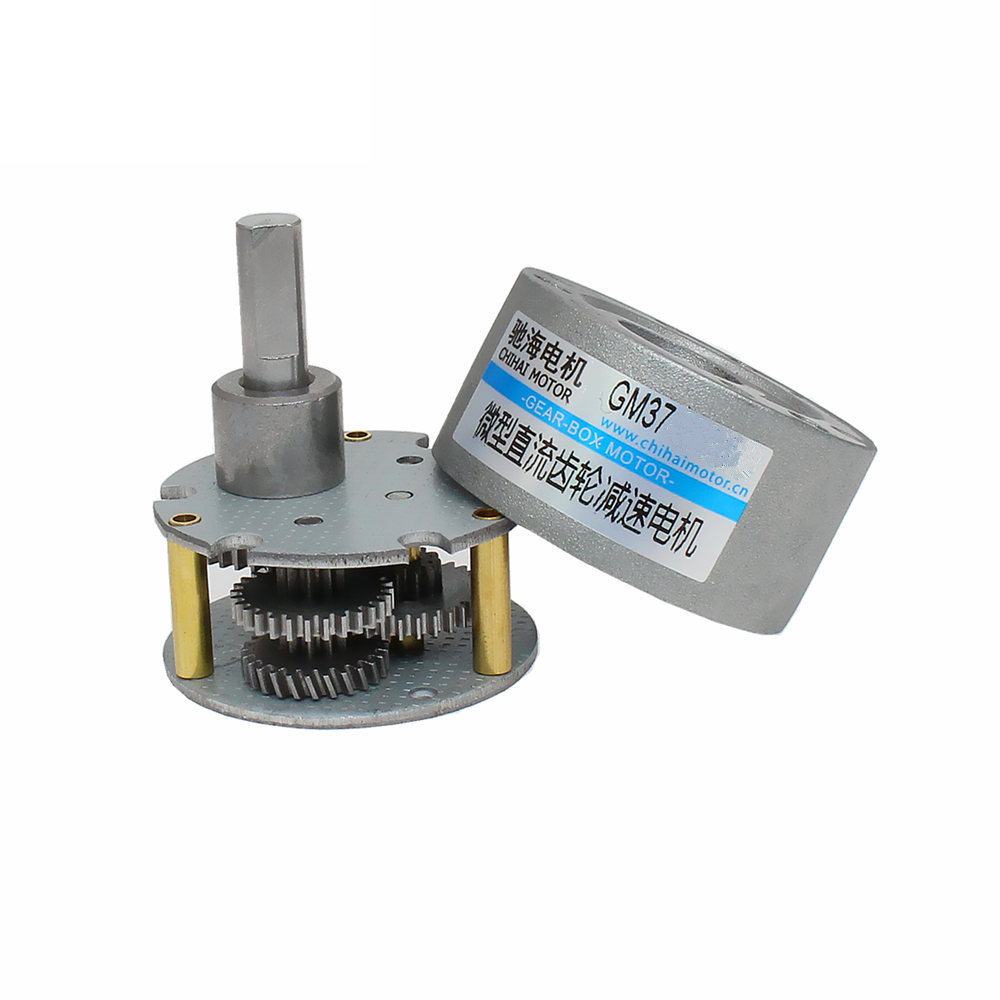
\includegraphics[width=2in]{4101_motor.jpg}
		% \caption{motor with reduction detail}\label{fig:4101}		
	\end{subfigure}
	\quad
	\begin{subfigure}
		\centering
		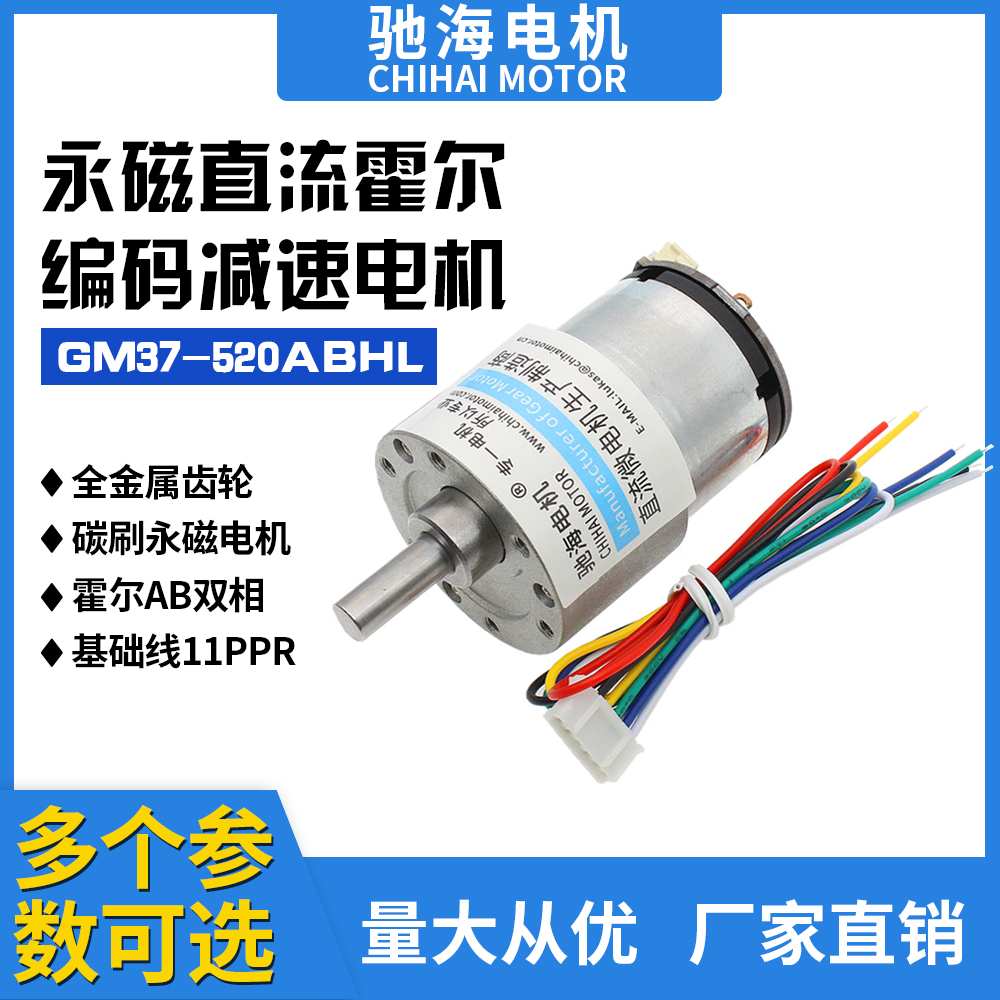
\includegraphics[width=2in]{4102_motor.jpg}
		% \caption{motor with brand}\label{fig:4102}
	\end{subfigure}
	\begin{subfigure}
		\centering
		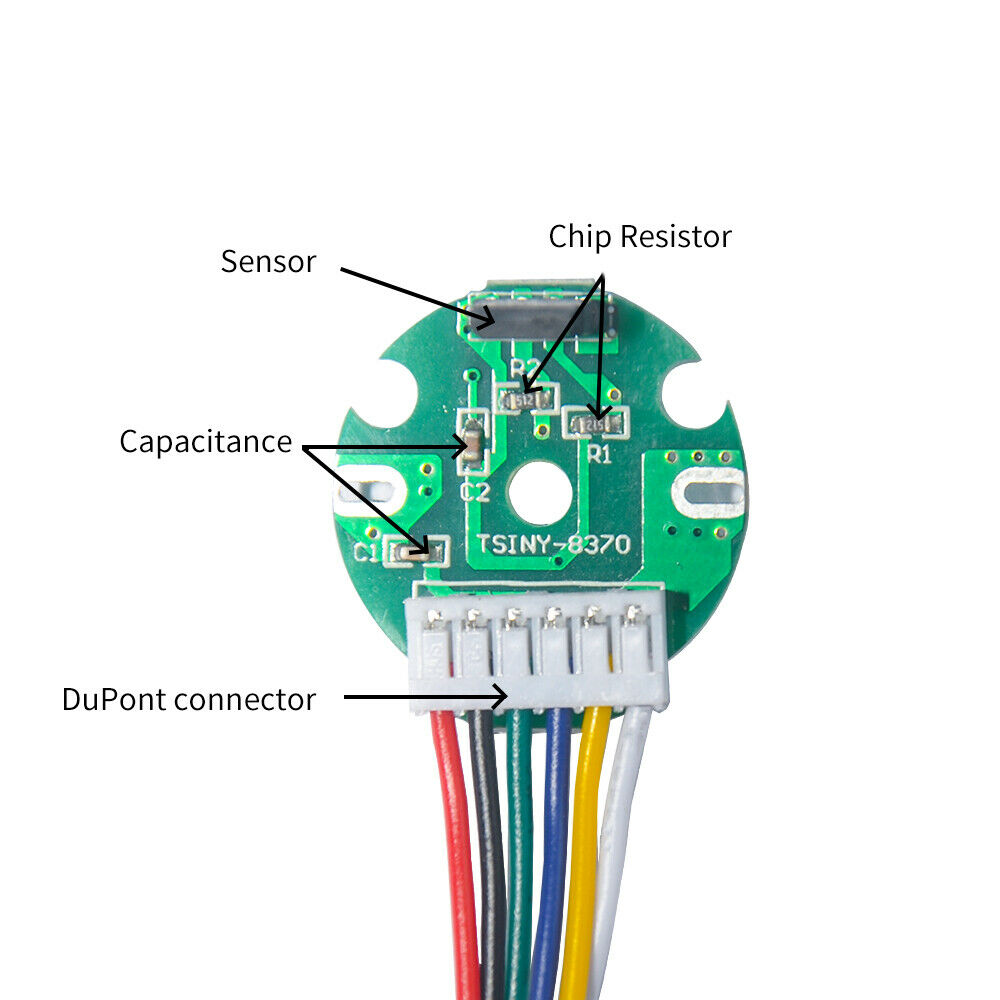
\includegraphics[width=2in]{412_hallencoder.jpg}
		% \caption{motor with brand}\label{fig:4102}
	\end{subfigure}
	\caption[Cleaning Motor]{ 
		Cleaning Motor: BLDC motor with Magnetic incremental hall encoder in cleaning unit.
		\href{https://www.ebay.com/itm/370-Motor-Hall-Encoder-DC-2-5V-24V-12-PPR-Dual-Quadrature-Outputs-Metal-Encoder/283429506020}
{370 magnetic Hall incremental encoder(MHIE) Pic Source} (here we use 520 MHIE) 		
			}\label{fig:410}
\end{figure}
% \marginnote[-12pt]{
% 	}

\section{Purchase Info}
\begin{enumerate}
	\item brand: CHIHAI MOTOR
	\item type: JGB37-520
	\item link: \href{https://item.taobao.com/item.htm?spm=a1z09.2.0.0.4a892e8d2d0m2a&id=531752422073&_u=i1s32jc02624}{taobao link} 
	\item price:  60RMB
	\item data: June. 2020
	\item RP: CZ, clear
\end{enumerate}

\section{Instruction for Connection}
wire definition in encoders:
\begin{enumerate}
	\item {\colorbox{red}W red}: M1, motor + positive
	\item {\colorbox{black}W black}: GND, encoder power supply - negative
	\item {\colorbox{yellow}W yellow}: C1, encoder signal A phase
	\item {\colorbox{green}W green}: C2, encoder signal B phase
	\item {\colorbox{blue}W blue}: 3.3/5v, encoder power supply + positive
	\item {\colorbox{white}W white}: M2, motor - negative 
\end{enumerate}

\section{Mechanical Specification}
It includes magnetic motor main part, reduction,  D shaft and a magnetic incremental encoder.

Motor specification:
\begin{enumerate}
	\item D shaft diameter: 6mm
	\item shaft length: 21mm, D part length: 12mm
	\item weight: 160g (different with the reduction ratio)
	\item L=24mm here
\end{enumerate}

\begin{figure}[htb]
	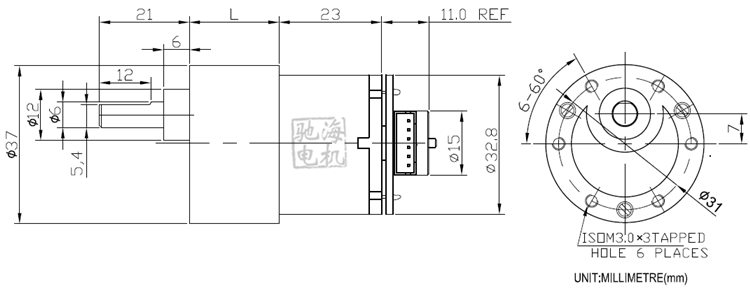
\includegraphics[width=1\textwidth]{411_motor_mechanical.jpg}
	\caption[Cleaning Motor mechanical specification]{ 
		Cleaning Motor electrical specification.		 
		}
	\labfig{fig412_hallencoder}
\end{figure}

\section{Electrical Specification}
Motor specification:
\begin{enumerate}
	\item voltage: 12v
	\item reduction ratio: 90 
	\item encoder resolution: 11* reduction ratio = 11*90=990
	\item speed w/o payload: 107rpm
	\item maximum output power: 7w
	\item nominal torque: 1.4N*m
\end{enumerate}

Encoder specification:
\begin{enumerate}
	\item type: AB biple phase incremental magnetic hall encoder
	\item power supply: 3.3v/5V
	\item frequency: 100KHZ
	\item basic pulse number: 11 PPR
	\item output signal: AB phase square wave
	\item interface: PH2.0
	\item directly connected to atom controller, self-included pulling resist
\end{enumerate}
\begin{figure}[htb]
	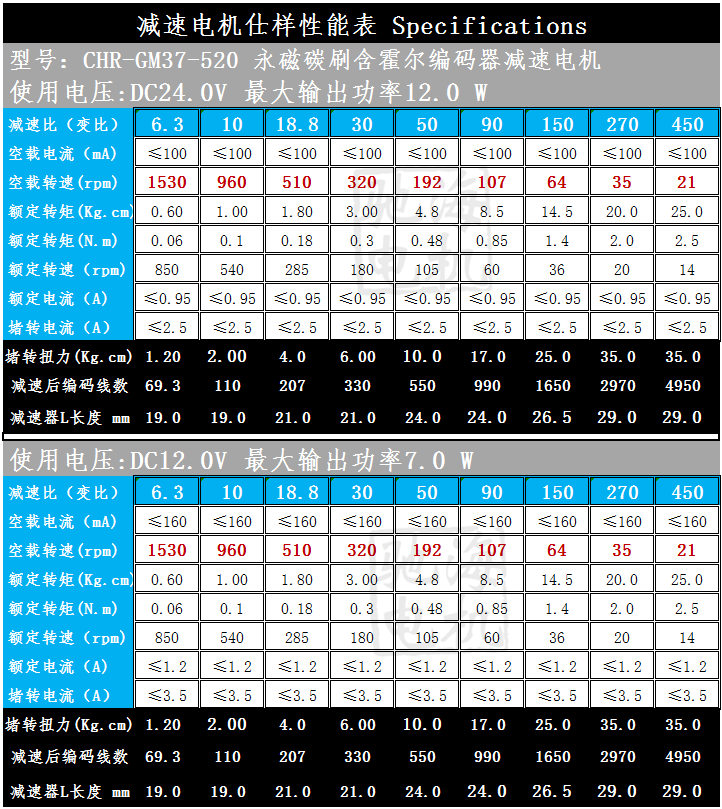
\includegraphics[width=0.8\textwidth]{413_el_specification}
	\caption[Cleaning Motor electrical specification]{ 
		Cleaning Motor electrical specification, here voltage is 12v, reduction ratio is 90.		 
		}
	\labfig{fig:413}
\end{figure}
